\documentclass{article} % Especially this!

%%%%%%%%%%%%%%%%%%%%%%%%%%%%%%%%%%%%%%%%%%%%%%%%%%%%%%%%

\usepackage[english]{babel}
\usepackage[utf8]{inputenc}
\usepackage[a4paper, total={6in, 8.5in}]{geometry}
\usepackage{amsmath}
\usepackage{amsthm}
\usepackage{amsfonts}
\usepackage{amssymb}
\usepackage[usenames,dvipsnames]{xcolor}
\usepackage{graphicx}
%\usepackage[siunitx]{circuitikz}
\usepackage{tikz}
\usepackage[colorinlistoftodos, color=orange!50]{todonotes}
\usepackage{hyperref}
\usepackage[numbers, square]{natbib}
\usepackage{fancybox}
\usepackage{epsfig}
\usepackage{soul}
\usepackage{listings}
\usepackage[framemethod=tikz]{mdframed}
\usepackage[shortlabels]{enumitem}
\usepackage[version=4]{mhchem}
\usepackage{multicol}
\usepackage{pgfplots}
\usepackage{version}
\pgfplotsset{compat=1.14}
\usepackage{graphicx}
\usepackage{subfig}

%%%%%%%%%%%%%%%%%%%%%%%%%%%%%%%%%%%%%%%%%%%%%%%%%%%%%%%

% SYNTAX FOR NEW COMMANDS:
%\newcommand{\new}{Old command or text}

% EXAMPLE:

\newcommand{\blah}{blah blah blah \dots}

\setlength{\marginparwidth}{3.4cm}


% NEW COUNTERS
\newcounter{points}
\setcounter{points}{100}
\newcounter{spelling}
\newcounter{english}
\newcounter{units}
\newcounter{other}
\newcounter{source}
\newcounter{concept}
\newcounter{missing}
\newcounter{math}
\newcounter{terms}
\newcounter{clarity}
\newcounter{late}

% COMMANDS
\newtheorem{theorem}{Theorem}

\newcommand{\late}{\todo{late submittal (-5)}
\addtocounter{late}{-5}
\addtocounter{points}{-5}}

\definecolor{pink}{RGB}{255,182,193}
\newcommand{\hlp}[2][pink]{ {\sethlcolor{#1} \hl{#2}} }

\definecolor{myblue}{rgb}{0.668, 0.805, 0.929}
\newcommand{\hlb}[2][myblue]{ {\sethlcolor{#1} \hl{#2}} }

\newcommand{\clarity}[2]{\todo[color=CornflowerBlue!50]{CLARITY of WRITING(#1) #2}\addtocounter{points}{#1}
\addtocounter{clarity}{#1}}

\newcommand{\other}[2]{\todo{OTHER(#1) #2} \addtocounter{points}{#1} \addtocounter{other}{#1}}

\newcommand{\spelling}{\todo[color=CornflowerBlue!50]{SPELLING (-1)} \addtocounter{points}{-1}
\addtocounter{spelling}{-1}}
\newcommand{\units}{\todo{UNITS (-1)} \addtocounter{points}{-1}
\addtocounter{units}{-1}}

\newcommand{\english}{\todo[color=CornflowerBlue!50]{SYNTAX and GRAMMAR (-1)} \addtocounter{points}{-1}
\addtocounter{english}{-1}}

\newcommand{\source}{\todo{SOURCE(S) (-2)} \addtocounter{points}{-2}
\addtocounter{source}{-2}}
\newcommand{\concept}{\todo{CONCEPT (-2)} \addtocounter{points}{-2}
\addtocounter{concept}{-2}}

\newcommand{\missing}[2]{\todo{MISSING CONTENT (#1) #2} \addtocounter{points}{#1}
\addtocounter{missing}{#1}}

\newcommand{\maths}{\todo{MATH (-1)} \addtocounter{points}{-1}
\addtocounter{math}{-1}}
\newcommand{\terms}{\todo[color=CornflowerBlue!50]{SCIENCE TERMS (-1)} \addtocounter{points}{-1}
\addtocounter{terms}{-1}}


\newcommand{\summary}[1]{
\begin{mdframed}[nobreak=true]
\begin{minipage}{\textwidth}
\vspace{0.5cm}
\begin{center}
\Large{Grade Summary} \hrule 
\end{center} \vspace{0.5cm}
General Comments: #1

\vspace{0.5cm}
Possible Points \dotfill 100 \\
Points Lost (Late Submittal) \dotfill \thelate \\
Points Lost (Science Terms) \dotfill \theterms \\
Points Lost (Syntax and Grammar) \dotfill \theenglish \\
Points Lost (Spelling) \dotfill \thespelling \\
Points Lost (Units) \dotfill \theunits \\
Points Lost (Math) \dotfill \themath \\
Points Lost (Sources) \dotfill \thesource \\
Points Lost (Concept) \dotfill \theconcept \\
Points Lost (Missing Content) \dotfill \themissing \\
Points Lost (Clarity of Writing) \dotfill \theclarity \\
Other \dotfill \theother \\[0.5cm]
\begin{center}
\large{\textbf{Grade:} \fbox{\thepoints}}
\end{center}
\end{minipage}
\end{mdframed}}

%#########################################################

%To use symbols for footnotes
\renewcommand*{\thefootnote}{\fnsymbol{footnote}}
%To change footnotes back to numbers uncomment the following line
%\renewcommand*{\thefootnote}{\arabic{footnote}}

% Enable this command to adjust line spacing for inline math equations.
% \everymath{\displaystyle}

%%%%%%%%%%%%%%%%%%%%%%%%%%%%%%%%%%%%%%%

\title{
\normalfont \normalsize 
\textsc{Physics of Complex Systems, 2021} \\ 
[10pt] 
\rule{\linewidth}{0.5pt} \\[6pt] 
\huge 
Simulation of a simple model of flocking
\rule{\linewidth}{2pt}  \\[10pt]
}
\author{Lorenzo Sani}
\date{\normalsize \today}

\begin{document}

\maketitle

\tableofcontents

%###############################################
\section{Abstract}
This short relation aims to show the results of the simulation of a simple model of flocking
in order to verify a theorem. At the same time, using the result of the simulation, it tries
to highlight the influence of the parameters of the model on the main characteristics of 
the flocking state.

%###############################################
\section{Introduction}
A common phenomena revealed by real complex systems is the emergence of a global 
behaviour in a system composed by many (sometimes identical) autonomous individuals or 
agents.
Physicists generally refer to emergence when the appearance of a global consensus cannot
be understood in the sense of the behaviours and laws of microscopic elements of a large
system; while refer to self-organization when the system reacts (or adapts) to external 
stimuli over time, and responds accordingly.
Examples of this behaviour can be found in many fields such economy, e.g. a 
common belief in a price system when activity takes place in a given market, or also
in biological systems, e.g. the way many animals moving together.
In this short relation it was simulated a simple model of flocking, where many birds,
with random initial positions and velocities, after some time assume the same velocity
and keep the same distances between each others. Having a global common velocity and 
keeping constant the relative distances, the birds reach a flocking state.

%###############################################
\section {The Model}
This short study is based on a model presented in \cite{CuckerSmale} . The authors considered 
a population of birds moving in $\mathbf{E}=\mathbf{R}^3$, and they
considered some empirical observations to model their dynamics.
In fact it has been observed that under some
initial conditions on positions and velocities of birds, 
the system of all the birds converges to one in which all them have the same velocity and 
stationary relative distances, i.e. the system fills a fixed volume.
Keeping this observations in mind, the authors of \cite{CuckerSmale} postulated a 
model for the evolution of the flock, which allows conditions under which the aimed convergence 
is reached. When these conditions are not satisfied the dispersion of birds is expected.

The proposed model postulates that every bird adjust its velocity by an additive term,
that is represented by the weighted average of the differences of its velocity with
those of all other birds. For the $i-th$ bird, the following holds:
\begin{equation}
	\label{eq1}
	v_i(t+h)-v_i(t)=h\sum_{j=1}^k a_{ij}(v_j(t)-v_i(t))
\end{equation}
In \eqref{eq1} $h$ represents the time step; the matrix whose elements are $a_{ij}$  is 
the weighting matrix; $k$ is the number of birds in the system. At this point it is 
useful to remark the fact that the interaction between birds is global, i.e. every bird
interacts with all the others. This is clearly a strong simplification of reality.
For complex network theorists, the matrix $\lbrace a_{ij}\rbrace$ can represent the adjacency
matrix $A_x$, where the subscript $x$ is referred to the space variable, of the graph
representing the set of birds. The graph represented by this adjacency matrix must be 
weighted, completely symmetric, and with non-zero constant diagonal.
Then, it is reasonable to assume that the weights $a_{ij}$ are functions of the (visual) 
perception that every bird has of all the others. It is assumed a quite simple function 
of the distance between birds that is a non-increasing function 
$\eta:\mathbf{R}^+\rightarrow\mathbf{R}^+$ such that
\begin{equation}
	\label{eq2}
	a_{ij}=\eta(x_i,x_j)=\frac{H}{(1+\left\Vert x_i - x_j \right\Vert^2)^{\beta}}
\end{equation}
for some fixed real values of $H>0$ and $\beta\geq0$. In \eqref{eq2} 
$\left\Vert \cdot \right\Vert$ represents the standard euclidean distance in our space 
$\mathbf{E}$. This function satisfies the properties requested by the graph.
We can write \eqref{eq1} in a more concise form by making use of some well-known 
properties of the adjacency matrix $A_x$, the degree matrix $D_x=diag(d_1,...,d_k)$, whose
elements are given by $d_i=\sum_{j\leq k}a_{ij}$ for $i=1,...,k$, 
and the Laplacian of $A_x$ defined by $L_x=D_x-A_x$. Then
\begin{align}
\label{eq3}
    v_i(t+h)-v_i(t)& = -h\sum_{j=1}^k a_{ij}(v_i(t)-v_j(t))\\
    & = -h\bigg(\sum_{j=1}^k a_{ij}\bigg)v_i(t)+h\sum_{j=1}^k \big(a_{ij}v_j(t)\big)\nonumber\\
    & = -h\lbrack D_xv(t)\rbrack_i+h\lbrack A_xv(t)\rbrack_i\nonumber\\
    & = -h\lbrack L_xv(t)\rbrack_i\nonumber
\end{align}
In \eqref{eq3} is crucial to remark that the notation $A_xv(t)$ does not refer to a 
$k \times k$ matrix acting on $\mathbf{R}^k$, but $A_x$ maps $(v_1, \dotsb ,v_k)$ 
to $(a_{i1}v_1+ \dotsb +a_{ik}v_k)_{i\leq k}$. The same holds for $D_x$ and $L_x$.
Adding a simple natural equation for the evolution of the positions, the following
system is obtained
\begin{align}
\label{eq4}
    &x(t+h) = x(t) + hv(t)\\
    &v(t+h) = (Id -hL_x)v(t)\nonumber
\end{align}
Here the notation is simplified by using $x(t)=\big(x_1(t),...,x_k(t)\big)$ and
$v(t)=\big(v_1(t),...,v_k(t)\big)$.
The paper \cite{CuckerSmale} proposed also the continuous version of \eqref{eq4}, that
is simply obtained by letting $h$ tend to zero. The following system of differential 
equations is then given.
\begin{align}
\label{eq5}
    &\dot{x} = v\\
    &\dot{v} = -L_xv\nonumber
\end{align}
Finally the authors of \cite{CuckerSmale} proved the following theorem
\begin{theorem}
    Let $x_0,y_0\in \mathbf{E}$. Then, there exists a unique solution $(x(t),v(t))$ of 
    \eqref{eq5}, defined for all $t \in \mathbf{R}$, with initial conditions $x(0)=x_0$ and
    $v(0)=v_0$. If $\beta<1/2$ then, when $t\rightarrow\infty$ the velocities $v_i(t)$ tend
    to a common limit $\widehat{v}\in\mathbf{E}$ and the vectors $x_i-x_j$ tend to a limit 
    vector $\widehat{x_{ij}}$, for all $i,j\leq k$. The same happens if $\beta\geq1/2$ provided
    the initial values $x_0$ and $v_0$ satisfy a given, explicit, relation.
\end{theorem}
Looking a bit deeper inside the model, by following the graph theory view, it is notable that
the Laplacian $L_x$ gives us many information about the structure of the graph $G$ described
by the adjacency matrix $A$. $L_x$ is symmetric, positive semi-definite and can be used to 
build the energy function of the flock. In fact, by noting that
\begin{equation}
	\label{eq6}
	\forall v \in \mathbf{E}^3, L_x(v,...,v)=0,
\end{equation} and
\begin{equation}
	\label{eq7}
	\langle L_xv,v\rangle=\frac{1}{2}\sum_{i,j=1}^ka_{ij}\left\Vert v_i - v_j\right\Vert^2,
\end{equation}
using the standard euclidean scalar product, we can define 
\begin{equation}
	\label{eq8}
	E_x(v)=2\langle L_xv,v\rangle=\sum_{i,j=1}^ka_{ij}\left\Vert v_i - v_j\right\Vert^2
\end{equation}
Now it turns clear that the results of the theorem imply the fact that for $t\rightarrow\infty$ $E_x(v)=0$,
since all the birds are flying with the same velocity. The physical interpretation of the 
convergence in the theorem relies on the minimization of the energy of the flock.

The question that
arises naturally is about how rapid is the convergence and how sharp is the critical value of $\beta=1/2$.
In \cite{CuckerSmale1} the authors give extended explanation on the 
discretization and assume, to maintain the validity of the theorem, one more constraint on
the function $\eta$ in \eqref{eq2}. They modified a bit the function to 
\begin{equation}
	\label{eq9}
	\eta(x_i,x_j)=\frac{H}{(\sigma^2+\left\Vert x_i - x_j \right\Vert^2)^{\beta}},
\end{equation}
where the new parameter $\sigma$ must be strictly positive, and they gave the constraint
\begin{equation}
	\label{eq10}
	H<\frac{\sigma^{2\beta}}{(k-1)\sqrt{k}},
\end{equation}
where $k$ is the number of birds in the flock.
Here $\sigma$ represent simply a scaling parameter. In fact letting by $X_i=\frac{x_i}{\sigma}$,
$\tau=\sigma^{-2\beta}t$, and $V_i=\frac{dX_i}{d\tau}=\sigma^{2\beta-1}v_i$,  the system becomes
\begin{align}
\label{eq11}
    \frac{dX_i}{d\tau} &= V_i\\
    \frac{dV_i}{d\tau} &= \sum_{i,j=1}^k\frac{H}{(1+\left\Vert X_i - X_j \right\Vert^2)^{\beta}}(V_i - V_j)\nonumber
\end{align}
The scaled systems has the same dynamics of the original one, but does not explicitly depend on $\sigma$.
Recalling the fact that $\sigma>0$ by definition, it is reasonable that, for different values of $\sigma$
and the same initial condition on $x$ and $v$, the system convergences to a flock with different features,
represented by its diameter and by the common velocity $\widehat{v}$. In particular for a value of $\beta<1/2$,
for which $2\beta-1<0$, one can expect to have for $\sigma\ll1$ higher values for the diameter and for $\widehat{v}$,
and viceversa for $\sigma\gg1$ lower values for the diameter and for $\widehat{v}$.


%###############################################
\section {Simulation}
The model described above was simulated in its discretized version in $\mathbf{E}=\mathbf{R}^3$.
A simple program written in \verb|C++| was used to simulate the model in order to allow the
tuning of the parameters.
A modular function, that accepts different values for the parameters of the model, was used.
The function is responsible of keeping the necessary constraints for reaching the convergence.
It receives as arguments the number of birds $k$, the value of $\beta$, the magnitude of the 
time step $h$, and the value of $\sigma$.
The initial conditions for the positions are taken by sampling the uniform 
distribution in the interval $[-5,5]$ for every component of every bird.
The same is done for the velocities.
The PRNG used is the Marsenne-Twister in \Verb|mt19937| class provided by the \verb|random| 
standard library.
The simulation proceeds as the following pseudo-code explains.
\begin{lstlisting}[language=C++]
applyInitialConditions(); // application of initial random conditions
do {
    computeAdjMatrix(); // compute the adjacency matrix
    computeAdjDegree(); // compute the degree matrix
    computeAdjLaplacian(); // compute the Laplacian matrix
    spatialDiffEq(); // apply the discrete differential equation for x
    velocityDiffEq(); // apply the discrete differential equation for v
} while (convergenceIsReached()) // convergence to the flocking state
\end{lstlisting}
In order to reach a good precision, the real variables have been represented by \verb|double|.

It is useful to spend some lines on the convergence criteria chosen. The main function defines
a maximum number of iteration the model should perform by taking \verb|max_iter = 50 * k|, where 
\verb|k| is the number of birds in the system. However the program allows to modify this value.
In real world the flocking state is reached very rapidly, but one has to 
consider that a bird can change its velocity in very short time.
The choice for the upper limit of the number of iteration means that a set of 10 birds should 
reach the flocking state at most in 500 time steps, that seems reasonable.
The other criteria are referred to the properties of the flocking state given by the Theorem.

For what concerns the velocity $\widehat{v}$, at every step are computed 
$v_a^{max} = \max_{i,j\in[0,k]}|v_{a,i} - v_{a,j}|$ where $a=1,2,3$, so that, when 
$\left\Vert v^{max}\right\Vert \rightarrow 0$ with
$v^{max} = (v_x^{max},v_y^{max},v_z^{max})$, the convergence to a state where all the birds 
have the same velocity is reached.

For what concerns the convergence to stationary displacements $\widehat{x_{ij}}$, at every 
step the displacements are computed component by component, such that 
$d_{a,ij}=x_{a,i}-x_{a,j}$ where $a=1,2,3$, and are then compared to the previous creating
a maximal difference vector in similar way to what has been done with the velocities.
It is computed $d_a^{max} = max_{ij\in\mathbf{A}}|d_{a,ij}^{t} - d_{a,ij}^{t-1}|$
where $a=1,2,3$ and $\mathbf{A}$ represents the set of all possible couples of birds.
Then, when $\left\Vert d^{max}\right\Vert \rightarrow 0$ with
$d^{max} = (d_x^{max},d_y^{max},d_z^{max})$, the convergence to a state where the relative
distances between birds becomes stationary.

The simulation evaluate at every iteration the value of both $v^{max}$ and $d^{max}$, and, 
if they are both lower than the acceptance value fixed at \verb|epsilon = 1.0e-5|, the simulation stops 
accepting the final state as the flocking state. Despite the model deals with point-like birds, 
this value seems a reasonable precision to be accepted.
However the program allows to modify the value of \verb|epsilon|.

%###############################################
\section {Results}
The focus of the simulation was in verifying the theorem and secondly
in underlying the dependence between the characteristics of the flocking state
and some of the parameters, especially $\sigma$, the scaling factor, and $k$, the number of
birds in the flock.

To verify the theorem were fixed the parameters $k=10$, $\sigma=1$. Then 200 simulations run with 
200 different values of $\beta\in[0,1]$ using a jump of 0.005, such that $\beta_{i+1}-\beta_i=0.005$.
The results are reported in Fig.\ref{fig1}, where $d^{max}$ and $v^{max}$ are plotted against the value
of beta. These show that the convergence to a flocking state is not so sharp. Testing different (reasonable) 
choices for the values of \verb|espilon| and \verb|max_iter| would change the value of $d^{max}$ and $v^{max}$
at $\beta=0.5$ but not the shape of $d^{max}(\beta)$ and $v^{max}(\beta)$  or the trend of convergence.
Up to now, the number of birds $k$ has not been taken into account. Taking \verb|max_iter = 50 * k| in 
all the following simulations, allows to reach the convergence to study the properties of the state, and 
implicitly states that with large values of $k$ the convergence is not reached without waiting long or 
relaxing a lot the value of \verb|epsilon|.
As Fig.\ref{fig4} shows, if the \verb|max_iter = 100| and \verb|espilon = 1e-5| are kept fixed and 
the number of birds $k$ is increased, the model does not converge exactly. The result of Fig.\ref{fig4} is that
maximal difference $d^{max}$ is of order unity as $v^{max}$ for higher value of $k$, while the requested precision
is \verb|espilon = 1e-5|.

The subsequent analysis of the results focuses on the role of $k$. The main question is about how 
the features of the flocking state change as functions of $k$. The flocking state is mainly
characterized by its global velocity $\widehat{v}$ and its diameter $D$, i.e. the maximum distance 
between two birds in the flock. There were simulated to this aim 200 systems with values of $k=2,...,202$ 
keeping fixed $\sigma=1$ and $\beta=0.4$.
As Fig.\ref{fig2}(a) shows, the diameter $D$ of the flocking state grows linearly with 
$k$, meaning that, 
while increasing $k$,
the displacements $\widehat{x_{ij}}$ have the same order of magnitude, as reality suggest.

As Fig.\ref{fig2}(b) shows, the norm of global velocity $\widehat{v}$ decays as $k$ grows, ensuring the stability 
of the flocking state, i.e. a large flock cannot go so fast although dispersion occurs and that is confirmed 
by the reality.

The last analysis focuses on the role of the scale parameter $\sigma$. The expectation is that 
the characteristics of the flocking state mentioned before change accordingly with $\sigma$. 
Recalling \eqref{eq11} and especially the change of coordinates that yields the new equations,
one can say that $\sigma=1$ represents a critical value, in some sense.
It is reasonable to expect one regime with higher $D$ and $\widehat{v}$ for $\sigma\ll1$, a regime 
with lower $D$ and $\widehat{v}$ for $\sigma\gg1$, and a regime with high variability for 
$D$ and $\widehat{v}$ both when $\sigma\thicksim 1$.
There were simulated to this aim 200 systems with values of $\sigma\in[10^{-5},10^5]$, almost 
uniformly distributed, while keeping fixed $k=10$ and $\beta=0.4$.
The dependence of the flocking state's features on $\sigma$ are shown in Fig.\ref{fig3},
where on the vertical axis are represented
the characteristics of the flocking state and in the horizontal axis the variable $\log\frac{1}{\sigma}$,
chosen to highlight the logistic shape of the relation. The results fulfill the expectation, but with a
larger range of variation that starts, as expected, at $\sigma=1$ reaching $\sigma=10^3$.

%###############################################
\section {Conclusions}
The results of these analysis give material to judge the applicability of this model to reality.

The dependence of the diameter $D$ and the common velocity $\widehat{v}$ of the flocking state 
on the number of birds $k$, seems to respect the observations. Moreover, at higher values of $k$,
in order to highlight these properties, it was necessary to relax a lot the convergence criteria. This suggest
that with very large values of $k$, the convergence is reached in a very long unreasonable time, 
and means that the model is not reliable.

The influence of $\sigma$ on the 
characteristics of the flocking state suggests that different, in the sense of $\sigma$, sets 
of birds should produce in the same way a flocking state, different in scale. The physical meaning of $\sigma$
could thus be related to a cognitive or language feature of birds' specie. 
Nature suggests that different bird's specie produce (or not) different flocking states. With this
point of view both $\sigma$ and $\beta$ could be seen as properties of the specie.

Finally the choice of the stopping criteria is fundamental. Increasing the parameter \verb|epsilon| ,
mentioned above, without increasing accordingly the \verb|max_iter| parameter, could produce 
systems with $\beta<1/2$ which cannot convergence to a flocking state, for these parameter.
Doing this is equivalent to ask for an unreasonable, or not so reasonable, convergence criteria.

The conclusion of this study is that, the model considered is a good starting point to produce 
systems with a flocking state and shows some interesting features when looking deeper in its parameters.
%###############################################
\section {Figures}
\begin{figure}[h!]
    \centering
    \subfloat[]{
        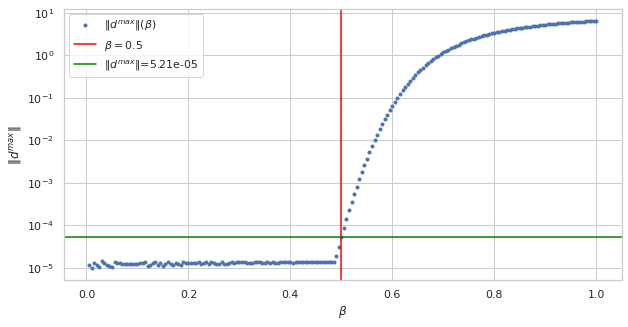
\includegraphics[width=0.45\textwidth, keepaspectratio]{../images/d_conv.png}
    }
    \subfloat[]{
        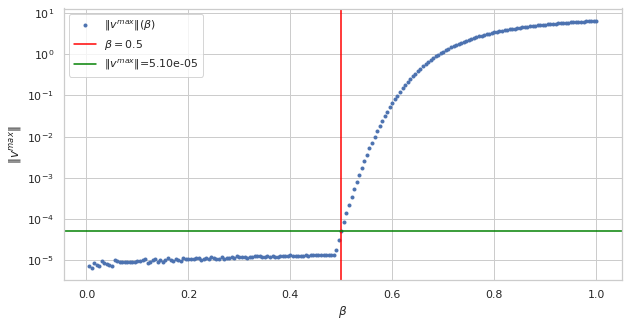
\includegraphics[width=0.45\textwidth, keepaspectratio]{../images/v_conv.png}
    }
    \caption{Here are shown the trends of the convergence for the topical case with $\sigma=1$ 
        and $k=100$. In (a) are plotted $\left\Vert d^{max}\right\Vert$ and in (b)
        $\left\Vert v^{max}\right\Vert$ both in logarithmic scale against
        different value of $\beta$. The red lines represent
        the value of $\beta=0.5$ in both. The green lines represent the value of 
        $\left\Vert d^{max}\right\Vert(\beta=0.5)$ in (a), and 
        $\left\Vert v^{max}\right\Vert(\beta=0.5)$ in (b).
        The vertical axis are in logarithmic scale.}
    \label{fig1}
\end{figure}
\begin{figure}[hb]
    \centering
    \subfloat[]{
        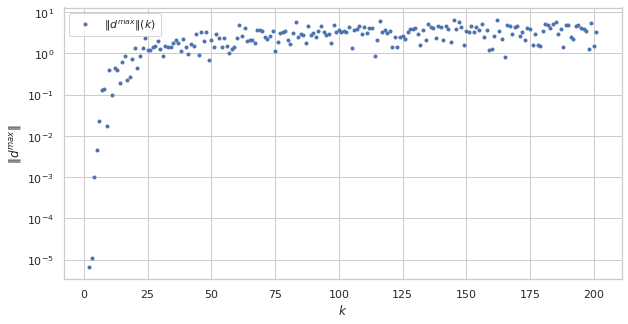
\includegraphics[width=0.45\textwidth, keepaspectratio]{../images/d_conv_N.png}
    }
    \subfloat[]{
        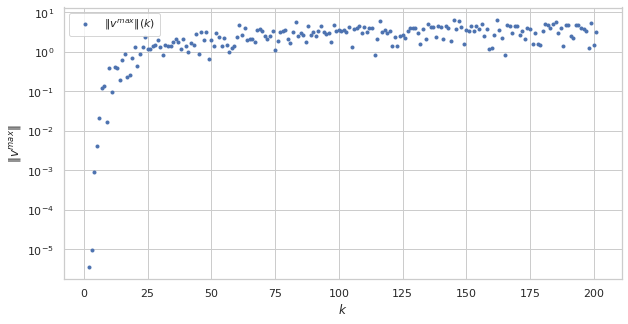
\includegraphics[width=0.45\textwidth, keepaspectratio]{../images/v_conv_N.png}
    }
    \caption{Here are shown the convergence values reached at the last iteration against the 
        number of birds $k$ of the model. The values for the convergence criteria 
         are kept fixed. The values of the parameters of the model are 
        kept fixed to $\sigma=1$, $\beta=0.5$, $k=10$.
        The vertical axis are in logarithmic scale. In (a) is plotted the convergence coefficient w.r.t.
        the distances, while in (b) the convergence coefficient w.r.t. the global velocity.}
    \label{fig4}
\end{figure}
\newpage
\begin{figure}[ht]
    \centering
    \subfloat[]{
        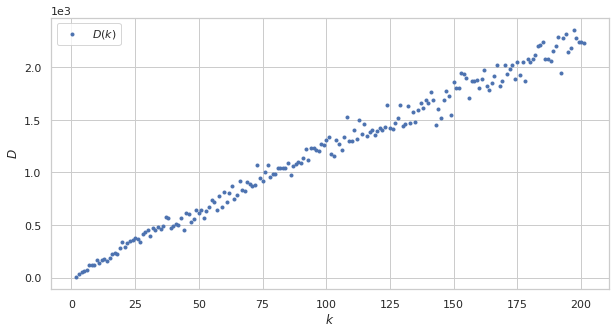
\includegraphics[width=0.45\textwidth, keepaspectratio]{../images/D_N.png}
    }
    \subfloat[]{
        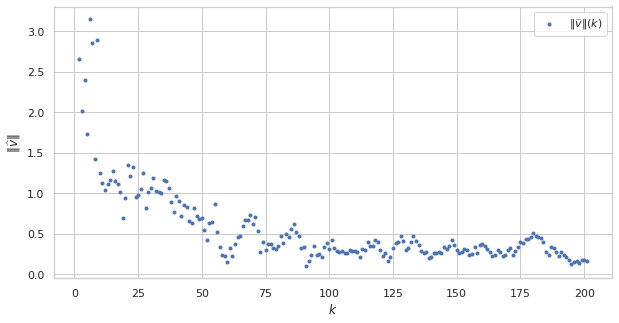
\includegraphics[width=0.45\textwidth, keepaspectratio]{../images/v_N.png}
    }
    \caption{Here is shown how the parameter $k$ influence the characteristics of the flocking state.
        This simulations run with $\sigma=1$ and $\beta=0.4$.
        In (a) is plotted the diameter $D$ of the flocking state versus the number of birds $k$.
        In (b) is plotted the norm of the global velocity $\widehat{v}$ of the flocking state 
        versus the number of birds $k$.}
    \label{fig2}
\end{figure}
\begin{figure}[ht]
    \centering
    \subfloat[]{
        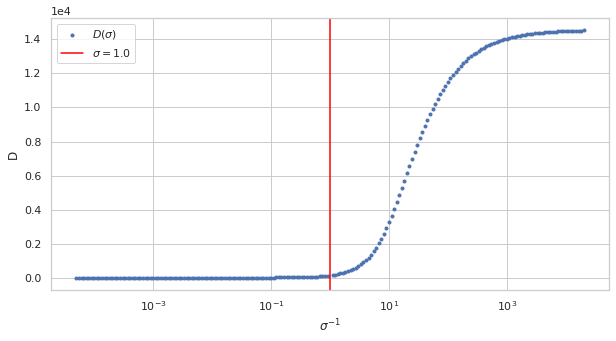
\includegraphics[width=0.45\textwidth, keepaspectratio]{../images/D_sigma.png}
    }
    \subfloat[]{
        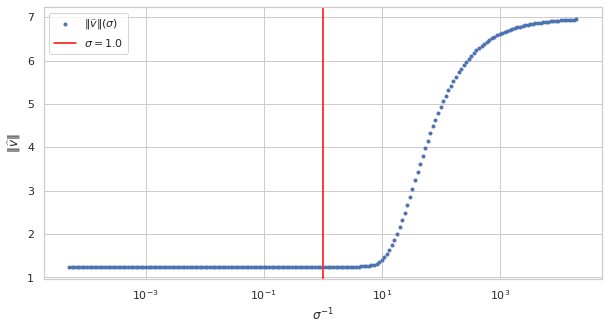
\includegraphics[width=0.45\textwidth, keepaspectratio]{../images/v_sigma.png}
    }
    \caption{Here is shown how the parameter $\sigma$ influence the characteristics of the flocking state.
    This simulations run with $k=10$ and $\beta=0.4$. The horizontal axis is in logarithmic scale.
    In (a) is plotted the diameter $D$ of the flocking state versus the value of the inverse of $\sigma$.
    In (b) is plotted the norm of the global velocity $\widehat{v}$ of the flocking state 
    versus the value of the inverse of $\sigma$.}
    \label{fig3}
\end{figure}
%###############################################

\section{Bibliography}
\begin{thebibliography}{90}
\bibitem{CuckerSmale}F. Cucker, S. Smale. "On the mathematics of emergence", The Mathematical Society of Japan and Springer 2007, Published online: 28 March 2007.
\bibitem{CuckerSmale1}F. Cucker, S. Smale. "Emergent Behaviour in Flocks", IEEE Transaction on Automatic Control, Vol. 52, No. 5, May 2007.
\bibitem{repo}\verb|https://github.com/relogu/PofCS_project|.
\end{thebibliography}

\newpage
\appendix
\renewcommand\thefigure{\thesection.\arabic{figure}}
\end{document} % NOTHING AFTER THIS LINE IS PART OF THE DOCUMENT